\documentclass[12pt, titlepage]{article}

\usepackage{fullpage}
\usepackage[round]{natbib}
\usepackage{multirow}
\usepackage{booktabs}
\usepackage{tabularx}
\usepackage{graphicx}
\usepackage{float}
\usepackage{longtable}
\usepackage{array}
\usepackage{xstring}
\usepackage{hyperref}
\hypersetup{
    colorlinks,
    citecolor=blue,
    filecolor=black,
    linkcolor=red,
    urlcolor=blue
}

\input{../../Comments.text}
\input{../../Common.text}

% Descriptive identifiers (same convention as the SRS and Hazard Analysis).
\newcommand{\descriptiveid}[1]{{\noexpandarg\StrSubstitute{#1}{_}{\textunderscore\allowbreak}[\idtmp]\texttt{\idtmp}}}
\newcommand{\idref}[1]{\hyperref[#1]{\descriptiveid{#1}}}
\newcommand{\idlabel}[1]{\descriptiveid{#1}}
\newcommand{\reqitem}[2]{\refstepcounter{#1}\label{#2}\idlabel{#2}}

% Link into the published SRS PDF.
\newcommand{\srsurl}{https://github.com/Ayushpatel2026/Keystone/raw/main/pdfs/SRS/SRS.pdf}
\newcommand{\srsref}[1]{\href{\srsurl\#nameddest=#1}{\descriptiveid{#1}}}

\newcounter{acnum} % anticipated change ordering
\newcommand{\actheacnum}{AC\theacnum}
\newcommand{\acref}[1]{\idref{#1}}

\newcounter{ucnum} % unlikely change ordering
\newcommand{\uctheucnum}{UC\theucnum}
\newcommand{\uref}[1]{\idref{#1}}

\newcounter{mnum}
\newcommand{\mthemnum}{M\themnum}
\newcommand{\mref}[1]{\idref{#1}}

\begin{document}

\title{Module Guide for \projname{}}
\author{\authname}
\date{\today}

\maketitle

\pagenumbering{roman}

\section{Revision History}

\begin{tabularx}{\textwidth}{p{3cm}p{2cm}X}
\toprule {\bf Date} & {\bf Version} & {\bf Notes}\\
\midrule
Nov. 12, 2026 & -1.0 & Added Revision -1 content: LC, UC, Modules, SRS Traceability\\
Nov. 13, 2026 & -1.1 & Addressed review for Rev -1 content\\
\bottomrule
\end{tabularx}

\newpage

\section{Reference Material}

This section records information for easy reference. 

\subsection{Abbreviations and Acronyms}

\renewcommand{\arraystretch}{1.2}
\begin{tabular}{l l} 
  \toprule		
  \textbf{symbol} & \textbf{description}\\
  \midrule 
  AC & Anticipated Change\\
  DAG & Directed Acyclic Graph \\
  FR & Functional Requirement\\
  \projname & Platform for capstone team formation and project selection\\
  LC & Likely Change (from the SRS)\\
  M & Module \\
  MG & Module Guide \\
  MGUC & Module Guide Unlikely Change \\
  NFR & Non-Functional Requirement\\
  OS & Operating System \\
  SRS & Software Requirements Specification\\
  SSO & Single Sign-On\\
  TA & Teaching Assistant\\
  UI & User Interface\\
  \wss{etc.} & \wss{...}\\
  \bottomrule
\end{tabular}\\

\newpage

\tableofcontents

\listoftables

\listoffigures

\newpage

\pagenumbering{arabic}

\section{Introduction}

Decomposing a system into modules is a commonly accepted approach to developing
software.  A module is a work assignment for a programmer or programming
team~\citep{ParnasEtAl1984}.  We advocate a decomposition
based on the principle of information hiding~\citep{Parnas1972a}.  This
principle supports design for change, because the ``secrets'' that each module
hides represent likely future changes.  Design for change is valuable in \projname{},
since each course may need different rules and processes.  

Our design follows the rules laid out by \citet{ParnasEtAl1984}, as follows:
\begin{itemize}
\item System details that are likely to change independently should be the
  secrets of separate modules.
\item Each data structure is implemented in only one module.
\item Any other program that requires information stored in a module's data
  structures must obtain it by calling access programs belonging to that module.
\end{itemize}

After completing the first stage of the design, the Software Requirements
Specification (SRS), the Module Guide (MG) is developed~\citep{ParnasEtAl1984}. The MG
specifies the modular structure of the system and is intended to allow both
designers and maintainers to easily identify the parts of the software.  The
potential readers of this document are as follows:

\begin{itemize}
\item New project members: This document can be a guide for a new project member
  to easily understand the overall structure and quickly find the
  relevant modules they are searching for.
\item Maintainers: The hierarchical structure of the module guide improves the
  maintainers' understanding when they need to make changes to the system. It is
  important for a maintainer to update the relevant sections of the document
  after changes have been made.
\item Designers: Once the module guide has been written, it can be used to
  check for consistency, feasibility, and flexibility. Designers can verify the
  system in various ways, such as consistency among modules, feasibility of the
  decomposition, and flexibility of the design.
\end{itemize}

The rest of the document is organized as follows. Section
\ref{SecChange} lists the anticipated and unlikely changes of the software
requirements. Section \ref{SecMH} summarizes the module decomposition that
was constructed according to the likely changes. Section \ref{SecConnection}
specifies the connections between the software requirements and the
modules. Section \ref{SecMD} gives a detailed description of the
modules. Section \ref{SecTM} includes three traceability matrices. Two check
the completeness of the design against the functional and non-functional
requirements in the SRS. The third shows the relation between anticipated
changes and the modules. Section
\ref{SecUse} describes the use relation between modules.

\section{Anticipated and Unlikely Changes} \label{SecChange}

This section lists possible changes to the system. According to the likeliness
of the change, the possible changes are classified into two
categories. Anticipated changes are listed in Section \ref{SecAchange}, and
unlikely changes are listed in Section \ref{SecUchange}.

\subsection{Anticipated Changes} \label{SecAchange}

Anticipated changes are the source of the information that is to be hidden
inside the modules. Ideally, changing one of the anticipated changes will only
require changing the one module that hides the associated decision. The approach
adapted here is called design for
change.

The anticipated changes below are a superset of the likely changes in the SRS
\citep{SRS}. Anticipated changes sourced directly from the SRS are identified.

\noindent \begin{itemize}
  \item[]\reqitem{acnum}{AC_Hardware}
  \textbf{Hardware Platform.}
  The operating system, browser, and container runtime on which \projname{} is
  run and accessed may change, for example a new hosting environment or new
  browser versions (\srsref{NFR_Browsers}, \srsref{NFR_Container}).
  \textit{Module:} \idref{M_HardwareHiding}.

  \item[]\reqitem{acnum}{AC_UserInterface}
  \textbf{User Interface.}
  The appearance, layout, and navigation of the platform's views may
  change, for example after usability testing.
  \textit{Module:} \idref{M_UserInterface}.

  \item[]\reqitem{acnum}{AC_SignInProcedure}
  \textbf{Sign-In Procedure.}
  How a user signs in, including the identity providers used (McMaster SSO and
  a provider for external supervisors) and the protocols for reaching them, and
  which actions require the user to re-authenticate, may change.
  \textit{SRS Likely Change:} \srsref{LC_SignIn}.
  \textit{Module:} \idref{M_Authentication}.

  \item[]\reqitem{acnum}{AC_RolePermissions}
  \textbf{Role Permissions.}
  What each role may see and do may change, and new roles may be added.
  \textit{SRS Likely Change:} \srsref{LC_Users}.
  \textit{Module:} \idref{M_Authorization}.

  \item[]\reqitem{acnum}{AC_CourseConfig}
  \textbf{Course Configuration.}
  The set of course features that can be switched on and off, and the course
  parameters an instructor can set, may change.
  \textit{SRS Likely Change:} \srsref{LC_CourseFeatures}.
  \textit{Module:} \idref{M_CourseManagement}.

  \item[]\reqitem{acnum}{AC_EnrollmentSource}
  \textbf{Enrollment Source.}
  Where enrollment data comes from (Avenue to Learn, an uploaded file), and the
  format it arrives in, may change.
  \textit{Module:} \idref{M_Enrollment}.

  \item[]\reqitem{acnum}{AC_ProposalTemplate}
  \textbf{Proposal Template.}
  The fields of a project proposal, and which of them are required or optional,
  may change and may differ between courses.
  \textit{SRS Likely Change:} \srsref{LC_ProposalTemplates}.
  \textit{Module:} \idref{M_Projects}.

  \item[]\reqitem{acnum}{AC_TeamFormation}
  \textbf{Team Formation.}
  How students form teams may change and may differ between courses. This
  includes the information collected in student and team profiles, and the
  rules a team must satisfy in a course (size limits, permitted program
  combinations, eligibility of students from other departments).
  \textit{SRS Likely Changes:} \srsref{LC_ProfileFields},
  \srsref{LC_TeamCourseRestrictions}.
  \textit{Module:} \idref{M_StudentsTeams}.

  \item[]\reqitem{acnum}{AC_Recommendation}
  \textbf{Recommendation Method.}
  How teammates, teams, and projects are matched may change, be extended to
  more criteria, or be removed.
  \textit{SRS Likely Change:} \srsref{LC_Recommendations}.
  \textit{Module:} \idref{M_Recommendation}.

  \item[]\reqitem{acnum}{AC_ApprovalWorkflow}
  \textbf{Approval Process.}
  The steps, approvers, and mode (in-platform, external, or integrated) by
  which a course approves team projects may change and may differ between
  courses. This includes the external system a course uses (e.g.: a GitLab
  merge request) and its interface.
  \textit{SRS Likely Change:} \srsref{LC_ApprovalWorkflows}.
  \textit{Module:} \idref{M_ApprovalWorkflow}.

  \item[]\reqitem{acnum}{AC_ThreadTargets}
  \textbf{Discussion Thread Targets.}
  Which records a discussion thread can be attached to, and how many threads
  each may have, may change.
  \textit{SRS Likely Change:} \srsref{LC_ThreadTargets}.
  \textit{Module:} \idref{M_Threads}.

  \item[]\reqitem{acnum}{AC_NotificationRules}
  \textbf{Notification Rules.}
  Which events cause a notification, and who receives it, may change.
  \textit{SRS Likely Change:} \srsref{LC_NotificationRules}.
  \textit{Module:} \idref{M_Notifications}.

  \item[]\reqitem{acnum}{AC_RequiredActions}
  \textbf{Required Actions.}
  Which actions appear on a user's checklist of required actions may change.
  \textit{SRS Likely Change:} \srsref{LC_RequiredActions}.
  \textit{Module:} \idref{M_Checklist}.

  \item[]\reqitem{acnum}{AC_Report}
  \textbf{Course Reports.}
  The contents of course reports, and the format they are exported in, may
  change.
  \textit{SRS Likely Change:} \srsref{LC_CourseReports}.
  \textit{Module:} \idref{M_CourseReport}.

  \item[]\reqitem{acnum}{AC_Persistence}
  \textbf{Data Storage.}
  The technology used to store \projname{}'s records, and how the records are
  laid out in it, may change.
  \textit{Module:} \idref{M_Persistence}.

  \item[]\reqitem{acnum}{AC_EmailService}
  \textbf{Email Service.}
  The service used to deliver email may change.
  \textit{Module:} \idref{M_EmailDelivery}.

  \item[]\reqitem{acnum}{AC_Audit}
  \textbf{Audit Records.}
  How audit records are stored at rest, including the
  tamper-evident mechanism, may change.
  \textit{Module:} \idref{M_AuditLog}.
\end{itemize}

\wss{Anticipated changes relate to changes that would be made in requirements,
design or implementation choices.  They are not related to changes that are made
at run-time, like the values of parameters.}

\subsection{Unlikely Changes} \label{SecUchange}

The module design should be as general as possible. However, a general system is
more complex. Sometimes this complexity is not necessary. Fixing some design
decisions at the system architecture stage can simplify the software design. If
these decision should later need to be changed, then many parts of the design
will potentially need to be modified. Hence, it is not intended that these
decisions will be changed.


\noindent \begin{itemize}
  \item[]\reqitem{ucnum}{MGUC_CoreRoles}
  \textbf{Core Roles.}
  The four core roles (Student, Supervisor, Instructor, and TA) will not change,
  since they are the primary users of the system.
  \textit{SRS Unlikely Change:} Core Stakeholder Roles.

  \item[]\reqitem{ucnum}{MGUC_HumanApproval}
  \textbf{Human Approval.}
  Approval decisions on proposals and team projects will always be made by a
  person, never automatically.
  \textit{SRS Unlikely Change:} Human-centered approval.

  \item[]\reqitem{ucnum}{MGUC_CourseOrganization}
  \textbf{Course Organization.}
  Students, instructors, TAs, projects, and teams will remain organized by
  course.
  \textit{SRS Unlikely Change:} Course Organization.

  \item[]\reqitem{ucnum}{MGUC_OverallFlow}
  \textbf{Overall Flow.}
  Students may browse projects at any time, with or without a team, and form
  teams based on their interests. A student must be in a team to apply for or
  propose a project, and the team's project is then approved.
  \textit{SRS Unlikely Change:} Vision and Overall Flow.

  \item[]\reqitem{ucnum}{MGUC_ProjectAssignment}
  \textbf{Project Assignment.}
  A project will move from proposal, to approval, to being open for
  applications, to being taken by teams. A team will apply to a project and
  then reach agreement with its supervisor. These states of a project and of an
  application will not change.

  \item[]\reqitem{ucnum}{MGUC_IO}
  \textbf{Input and Output Devices.}
  Input will come from users through a web browser (keyboard, pointer, and
  uploaded files), and output will go to the browser screen and to email.

  \item[]\reqitem{ucnum}{MGUC_WebDelivery}
  \textbf{Web Delivery.}
  \projname{} will be delivered as a web application, with a user interface in
  the browser and the rest of the system on a server.

  \item[]\reqitem{ucnum}{MGUC_SingleInstitution}
  \textbf{Single Institution.}
  Each deployment of \projname{} will serve one institution.
\end{itemize}

\section{Module Hierarchy} \label{SecMH}

This section provides an overview of the module design. Modules are summarized
in a hierarchy decomposed by secrets in Table \ref{TblMH}. The modules listed
below, which are leaves in the hierarchy tree, are the modules that will
actually be implemented.

\begin{description}
\item [\idref{M_HardwareHiding}:] Hardware-Hiding Module
\item [\idref{M_UserInterface}:] User Interface Module
\item [\idref{M_Authentication}:] Authentication Module
\item [\idref{M_Authorization}:] Authorization Module
\item [\idref{M_CourseManagement}:] Course Management Module
\item [\idref{M_Enrollment}:] Enrollment Module
\item [\idref{M_Projects}:] Projects Module
\item [\idref{M_StudentsTeams}:] Students and Teams Module
\item [\idref{M_Recommendation}:] Recommendation Module
\item [\idref{M_ApprovalWorkflow}:] Approval Workflow Module
\item [\idref{M_Threads}:] Threads Module
\item [\idref{M_Notifications}:] Notifications Module
\item [\idref{M_Checklist}:] Checklist Module
\item [\idref{M_CourseReport}:] Course Report Module
\item [\idref{M_Persistence}:] Persistence Module
\item [\idref{M_EmailDelivery}:] Email Delivery Module
\item [\idref{M_AuditLog}:] Audit Log Module
\end{description}


\begin{table}[H]
\centering
\begin{tabular}{p{0.3\textwidth} p{0.6\textwidth}}
\toprule
\textbf{Level 1} & \textbf{Level 2}\\
\midrule

{Hardware-Hiding Module} & \idref{M_HardwareHiding} \\
\midrule

\multirow{13}{0.3\textwidth}{Behaviour-Hiding Module} & \idref{M_UserInterface}\\
 & \idref{M_Authentication}\\
 & \idref{M_Authorization}\\
 & \idref{M_CourseManagement}\\
 & \idref{M_Enrollment}\\
 & \idref{M_Projects}\\
 & \idref{M_StudentsTeams}\\
 & \idref{M_Recommendation}\\
 & \idref{M_ApprovalWorkflow}\\
 & \idref{M_Threads}\\
 & \idref{M_Notifications}\\
 & \idref{M_Checklist}\\
 & \idref{M_CourseReport}\\
\midrule

\multirow{3}{0.3\textwidth}{Software Decision Module} & \idref{M_Persistence}\\
 & \idref{M_EmailDelivery}\\
 & \idref{M_AuditLog}\\
\bottomrule

\end{tabular}
\caption{Module Hierarchy}
\label{TblMH}
\end{table}

\section{Connection Between Requirements and Design} \label{SecConnection}

The design of the system is intended to satisfy the requirements developed in
the SRS. In this stage, the system is decomposed into modules. The connection
between requirements and modules is listed in Table~\ref{TblRT}.

\wss{The intention of this section is to document decisions that are made
  ``between'' the requirements and the design.  To satisfy some requirements,
  design decisions need to be made.  Rather than make these decisions implicit,
  they are explicitly recorded here.  For instance, if a program has security
  requirements, a specific design decision may be made to satisfy those
  requirements with a password.}

The design decisions made to satisfy the requirements are:

\begin{itemize}
  \item \textbf{Access checks.} Every user signs in through
  \idref{M_Authentication} before doing anything, and every action is checked by
  \idref{M_Authorization} against the user's role in that course
  (\srsref{NFR_Authenticate}, \srsref{NFR_Authorize},
  \srsref{FR_AuthorizationRBAC}).

  \item \textbf{Supervisor verification as a role.} An unverified external
  supervisor holds a separate role. Verifying them is a role change in
  \idref{M_Authorization}, so all access rules stay in one module
  (\srsref{FR_ExternalSupervisorVerification},
  \srsref{FR_ExternalSupervisorScope}).

  \item \textbf{Course settings as data.} Each course's enabled features and
  settings are stored as data in \idref{M_CourseManagement}, not written into the
  code. This lets a feature be turned off on a live system
  (\srsref{FR_DisableFeatures}, \srsref{NFR_LiveDisable}).

  \item \textbf{External services hidden by the module that uses them.} Each
  outside system is reached only through the one module that needs it: identity
  providers through \idref{M_Authentication}, the external approval system
  through \idref{M_ApprovalWorkflow}, the enrollment source through
  \idref{M_Enrollment}, and the email service through \idref{M_EmailDelivery}.
  Replacing an outside system therefore changes one module
  (\srsref{FR_MacSSO}, \srsref{FR_ExternalApproval},
  \srsref{FR_ImportEnrollment}).

  \item \textbf{Stored notifications.} A notification is stored before it is
  sent, and \idref{M_Notifications} retries it until delivery is confirmed
  (\srsref{FR_DurableNotifications}, \srsref{FR_ActionRequiredEmail}).

  \item \textbf{One audit log.} User actions and errors from external services
  are all recorded through \idref{M_AuditLog}, which hides how the records are
  made tamper-evident (\srsref{NFR_AuditLog}, \srsref{NFR_AuditTamper},
  \srsref{FR_LogExternalErrors}).

  \item \textbf{One path to storage.} All records are saved and read through
  \idref{M_Persistence}, which handles concurrent changes, encryption at rest,
  and backups (\srsref{NFR_ConcurrencySafety}, \srsref{NFR_EncryptRest},
  \srsref{NFR_Recoverable}). All changes resulting from one user action are
  saved in a single transaction: either all of them are saved or none are. For
  example, rejecting a team's project and releasing the project slot reserved
  for that team either both succeed or neither is saved.

  \item \textbf{Passwords never stored in plain text.} Passwords are only
  stored as hashes, produced inside \idref{M_Authentication}
  (\srsref{NFR_PasswordHash}).

  \item \textbf{Encrypted connections.} The user interface and the server talk
  only over an encrypted (HTTPS) connection, provided by the web framework and
  operating system behind \idref{M_HardwareHiding}
  (\srsref{NFR_EncryptTransit}).

  \item \textbf{Web application.} The user interface runs in the browser and
  the rest of the system runs on a server (\idref{MGUC_WebDelivery}), so the
  system works on any supported browser and screen size
  (\srsref{NFR_Browsers}, \srsref{NFR_ScreenSize}).
\end{itemize}

\section{Module Decomposition} \label{SecMD}

Modules are decomposed according to the principle of ``information hiding''
proposed by \citet{ParnasEtAl1984}. The \emph{Secrets} field in a module
decomposition is a brief statement of the design decision hidden by the
module. The \emph{Services} field specifies \emph{what} the module will do
without documenting \emph{how} to do it. For each module, a suggestion for the
implementing software is given under the \emph{Implemented By} title. If the
entry is \emph{OS}, this means that the module is provided by the operating
system or by standard programming language libraries.  \emph{\projname{}} means the
module will be implemented by the \projname{} software.

Only the leaf modules in the hierarchy have to be implemented. If a dash
(\emph{--}) is shown, this means that the module is not a leaf and will not have
to be implemented.

\subsection[Hardware-Hiding Module]{Hardware-Hiding Module (\protect\descriptiveid{M_HardwareHiding})}\label{M_HardwareHiding}

\begin{description}
\item[Secrets:] The platform the system runs on.
\item[Services:] Serves as a virtual hardware used by the rest of the system, so the system can accept input, display output, store files, and make network connections, including encrypted (HTTPS) connections between the browser and the server.
\item[Implemented By:] OS
\end{description}

\subsection{Behaviour-Hiding Module}

\begin{description}
\item[Secrets:]The contents of the required behaviours.
\item[Services:]Includes programs that provide externally visible behaviour of
  the system as specified in the software requirements specification (SRS)
  documents. This module serves as a communication layer between the
  hardware-hiding module and the software decision module. Changes in the SRS
  will need to be reflected here.
\item[Implemented By:] --
\end{description}

\wss{Template example of a leaf module. Input Format Module: Secrets: The format and structure of the input data. Services: Converts the input data into the data structure used by the input parameters module. Implemented By: [Your Program Name Here]. Type of Module: [Record, Library, Abstract Object, or Abstract Data Type] [Information to include for leaf modules in the decomposition by secrets tree.]}

\subsubsection[User Interface Module]{User Interface Module (\protect\descriptiveid{M_UserInterface})}\label{M_UserInterface}

\begin{description}
\item[Secrets:] The design of each view.
\item[Services:] Shows information to the user and collects their input for every user task.
\item[Implemented By:] \projname{}
\item[Type of Module:] Abstract Object
\end{description}

\subsubsection[Authentication Module]{Authentication Module (\protect\descriptiveid{M_Authentication})}\label{M_Authentication}

\begin{description}
\item[Secrets:] How a user is identified and verified.
\item[Services:] Signs users in through McMaster SSO or the provider used by external supervisors, keeps each user's identity (name, email, and linked sign-in account), stores passwords only as hashes and checks passwords against them, and re-verifies users before high-risk actions.
\item[Implemented By:] \projname{}
\item[Type of Module:] Abstract Object
\end{description}

\subsubsection[Authorization Module]{Authorization Module (\protect\descriptiveid{M_Authorization})}\label{M_Authorization}

\begin{description}
\item[Secrets:] What each user is allowed to do.
\item[Services:] Records, changes, and looks up each user's role, and decides whether a user may take an action or see a record based on that role. An unverified external supervisor holds a separate role, so verifying them is a role change.
\item[Implemented By:] \projname{}
\item[Type of Module:] Abstract Object
\end{description}

\subsubsection[Course Management Module]{Course Management Module (\protect\descriptiveid{M_CourseManagement})}\label{M_CourseManagement}

\begin{description}
\item[Secrets:] The setup of each course.
\item[Services:] Stores each course's settings and enabled features, keeps track of which features have pending work, and refuses to turn off a feature that has pending work. Lets instructors and TAs publish and update course material, and lets students and supervisors read it.
\item[Implemented By:] \projname{}
\item[Type of Module:] Abstract Object
\end{description}

\subsubsection[Enrollment Module]{Enrollment Module (\protect\descriptiveid{M_Enrollment})}\label{M_Enrollment}

\begin{description}
\item[Secrets:] How a course's student list is obtained.
\item[Services:] Reads an enrollment list from Avenue to Learn or an uploaded file, previews it against the current course list, applies it after confirmation, adds single students, and flags students missing from the latest list.
\item[Implemented By:] \projname{}
\item[Type of Module:] Abstract Object
\end{description}

\subsubsection[Projects Module]{Projects Module (\protect\descriptiveid{M_Projects})}\label{M_Projects}

\begin{description}
\item[Secrets:] The project records and their life cycle.
\item[Services:] Gives the proposal form for a course and checks that a proposal has every required field. Records proposals and their review, tracks how many teams a project can take, and records team applications, supervisor decisions, and agreements. Reserves and releases project slots, and withdraws competing applications when a team reaches agreement. Returns the projects a user may see, searched, filtered, and sorted as requested.
\item[Implemented By:] \projname{}
\item[Type of Module:] Abstract Object
\end{description}

\subsubsection[Students and Teams Module]{Students and Teams Module (\protect\descriptiveid{M_StudentsTeams})}\label{M_StudentsTeams}

\begin{description}
\item[Secrets:] How students form teams.
\item[Services:] Creates, updates, and shows student and team profiles. Creates teams, handles invitations and joining, records member roles and the assigned TA, and lists students without a team. Stores each course's team rules, checks a team against them, and reports any rule it breaks.
\item[Implemented By:] \projname{}
\item[Type of Module:] Abstract Object
\end{description}

\subsubsection[Recommendation Module]{Recommendation Module (\protect\descriptiveid{M_Recommendation})}\label{M_Recommendation}

\begin{description}
\item[Secrets:] The method used to match students, teams, and projects.
\item[Services:] Suggests teammates, teams, and projects for a student or team.
\item[Implemented By:] \projname{}
\item[Type of Module:] Library
\end{description}

\subsubsection[Approval Workflow Module]{Approval Workflow Module (\protect\descriptiveid{M_ApprovalWorkflow})}\label{M_ApprovalWorkflow}

\begin{description}
\item[Secrets:] The approval process of each course.
\item[Services:] Checks a submission before it is sent, sends it to the approvers (in the platform or in an external system such as a GitLab merge request), and records their decision. Handles changes to approved projects without replacing the existing approval until the changes are accepted.
\item[Implemented By:] \projname{}
\item[Type of Module:] Abstract Object
\end{description}

\subsubsection[Threads Module]{Threads Module (\protect\descriptiveid{M_Threads})}\label{M_Threads}

\begin{description}
\item[Secrets:] The records that discussion threads can be attached to.
\item[Services:] Creates threads on records that allow them, adds replies, and lists a record's threads.
\item[Implemented By:] \projname{}
\item[Type of Module:] Abstract Object
\end{description}

\subsubsection[Notifications Module]{Notifications Module (\protect\descriptiveid{M_Notifications})}\label{M_Notifications}

\begin{description}
\item[Secrets:] How users are notified of events.
\item[Services:] Decides who to notify about each event, writes the message, and keeps it until delivery is confirmed. Runs timed work, such as deadline reminders and retries of undelivered notifications.
\item[Implemented By:] \projname{}
\item[Type of Module:] Abstract Object
\end{description}

\subsubsection[Checklist Module]{Checklist Module (\protect\descriptiveid{M_Checklist})}\label{M_Checklist}

\begin{description}
\item[Secrets:] How a user's required actions are worked out.
\item[Services:] Lists a user's required actions and whether each one is done.
\item[Implemented By:] \projname{}
\item[Type of Module:] Library
\end{description}

\subsubsection[Course Report Module]{Course Report Module (\protect\descriptiveid{M_CourseReport})}\label{M_CourseReport}

\begin{description}
\item[Secrets:] The course report format.
\item[Services:] Shows instructors and TAs the status of projects, teams, and supervisors in their courses, and exports a report.
\item[Implemented By:] \projname{}
\item[Type of Module:] Library
\end{description}


\subsection{Software Decision Module}

\begin{description}
\item[Secrets:] The design decision based on mathematical theorems, physical
  facts, or programming considerations. The secrets of this module are
  \emph{not} described in the SRS.
\item[Services:] Includes data structure and algorithms used in the system that
  do not provide direct interaction with the user. 
  % Changes in these modules are more likely to be motivated by a desire to
  % improve performance than by externally imposed changes.
\item[Implemented By:] --
\end{description}

\subsubsection[Persistence Module]{Persistence Module (\protect\descriptiveid{M_Persistence})}\label{M_Persistence}

\begin{description}
\item[Secrets:] How records are stored.
\item[Services:] Saves, reads, and changes records safely when several users act at once, saving all changes from one user action in a single transaction, keeps records encrypted, and restores them from backups.
\item[Implemented By:] \projname{} (on PostgreSQL)
\item[Type of Module:] Abstract Object
\end{description}

\subsubsection[Email Delivery Module]{Email Delivery Module (\protect\descriptiveid{M_EmailDelivery})}\label{M_EmailDelivery}

\begin{description}
\item[Secrets:] How email is sent.
\item[Services:] Sends an email and reports whether it was delivered.
\item[Implemented By:] \projname{}
\item[Type of Module:] Abstract Object
\end{description}

\subsubsection[Audit Log Module]{Audit Log Module (\protect\descriptiveid{M_AuditLog})}\label{M_AuditLog}

\begin{description}
\item[Secrets:] How audit records are kept.
\item[Services:] Records each user action and each error from an external service, and lets authorized users read the records.
\item[Implemented By:] \projname{}
\item[Type of Module:] Abstract Object
\end{description}

\section{Traceability Matrix} \label{SecTM}

This section shows three traceability matrices: between the modules and the
functional requirements, the non-functional requirements, and the anticipated
changes.

% the table should use mref, the requirements should be named, use something
% like fref
\begin{longtable}{p{0.45\textwidth} p{0.50\textwidth}}

  \toprule
  Functional Requirement & Modules \\
  \midrule
  \srsref{FR_SupervisorProposal} & \idref{M_Projects} \\ \hline
  \srsref{FR_ProposalOptionalFields} & \idref{M_Projects} \\ \hline
  \srsref{FR_StudentProposal} & \idref{M_Projects} \\ \hline
  \srsref{FR_ReviewProposal} & \idref{M_Projects} \\ \hline
  \srsref{FR_ViewApprovedProjects} & \idref{M_Projects} \\ \hline
  \srsref{FR_ViewProjectStatus} & \idref{M_Projects} \\ \hline
  \srsref{FR_StudentProfile} & \idref{M_StudentsTeams} \\ \hline
  \srsref{FR_StudentTeams} & \idref{M_StudentsTeams} \\ \hline
  \srsref{FR_ValidateTeamRules} & \idref{M_StudentsTeams} \\ \hline
  \srsref{FR_TeamDiscovery} & \idref{M_StudentsTeams} \\ \hline
  \srsref{FR_TeamProfile} & \idref{M_StudentsTeams} \\ \hline
  \srsref{FR_TeamRecommend} & \idref{M_Recommendation} \\ \hline
  \srsref{FR_ProjectInterest} & \idref{M_Projects} \\ \hline
  \srsref{FR_DeclineTeam} & \idref{M_Projects} \\ \hline
  \srsref{FR_ProjectThreads} & \idref{M_Threads} \\ \hline
  \srsref{FR_ThreadsNotify} & \idref{M_Notifications}, \idref{M_EmailDelivery} \\ \hline
  \srsref{FR_RequestApproval} & \idref{M_ApprovalWorkflow} \\ \hline
  \srsref{FR_ApprovalResponse} & \idref{M_ApprovalWorkflow} \\ \hline
  \srsref{FR_ExternalApproval} & \idref{M_ApprovalWorkflow} \\ \hline
  \srsref{FR_ApprovalPreflightValidate} & \idref{M_ApprovalWorkflow}, \idref{M_StudentsTeams} \\ \hline
  \srsref{FR_ApprovalRevision} & \idref{M_ApprovalWorkflow} \\ \hline
  \srsref{FR_DisableFeatures} & \idref{M_CourseManagement} \\ \hline
  \srsref{FR_ReferenceMaterial} & \idref{M_CourseManagement} \\ \hline
  \srsref{FR_RequiredActionsList} & \idref{M_Checklist} \\ \hline
  \srsref{FR_ActionRequiredEmail} & \idref{M_Notifications}, \idref{M_Checklist}, \idref{M_EmailDelivery} \\ \hline
  \srsref{FR_ReadCourseInformation} & \idref{M_CourseReport} \\ \hline
  \srsref{FR_ExportCourseInformation} & \idref{M_CourseReport} \\ \hline
  \srsref{FR_MacSSO} & \idref{M_Authentication} \\ \hline
  \srsref{FR_AuthorizationRBAC} & \idref{M_Authorization} \\ \hline
  \srsref{FR_UpdateRoles} & \idref{M_Authorization} \\ \hline
  \srsref{FR_ExternalSupervisorVerification} & \idref{M_Authorization}, \idref{M_Authentication} \\ \hline
  \srsref{FR_ExternalSupervisorScope} & \idref{M_Authorization} \\ \hline
  \srsref{FR_LogExternalErrors} & \idref{M_AuditLog}, \idref{M_Notifications} \\ \hline
  \srsref{FR_RejectComponentDisable} & \idref{M_CourseManagement} \\ \hline
  \srsref{FR_DisplayTimestamps} & \idref{M_UserInterface}, \idref{M_Persistence} \\ \hline
  \srsref{FR_DurableNotifications} & \idref{M_Notifications} \\ \hline
  \srsref{FR_ReverifyUsers} & \idref{M_Authentication} \\ \hline
  \srsref{FR_ImportEnrollment} & \idref{M_Enrollment} \\ \hline
  \srsref{FR_UpdateEnrollment} & \idref{M_Enrollment} \\ \hline
  \srsref{FR_EnrollmentDiscrepency} & \idref{M_Enrollment} \\ \hline
  \srsref{FR_NeedsGroup} & \idref{M_StudentsTeams} \\ \hline
  \srsref{FR_AssignTA} & \idref{M_StudentsTeams} \\ \hline

  \bottomrule

  \caption{Trace Between Functional Requirements and Modules}
  \label{TblRT}
\end{longtable}

\begin{longtable}{p{0.45\textwidth} p{0.50\textwidth}}

  \toprule
  Non-Functional Requirement & Modules \\
  \midrule
  \srsref{NFR_ScreenSize} & \idref{M_UserInterface} \\ \hline
  \srsref{NFR_UsabilityFirstSuccess} & \idref{M_UserInterface} \\ \hline
  \srsref{NFR_LearnUnassisted} & \idref{M_UserInterface} \\ \hline
  \srsref{NFR_AccessibilityWCAG} & \idref{M_UserInterface} \\ \hline
  \srsref{NFR_PerfTail} & \idref{M_HardwareHiding}, \idref{M_Persistence} \\ \hline
  \srsref{NFR_Uptime} & \idref{M_HardwareHiding} \\ \hline
  \srsref{NFR_Recoverable} & \idref{M_Persistence} \\ \hline
  \srsref{NFR_PeakUsers} & \idref{M_HardwareHiding}, \idref{M_Persistence} \\ \hline
  \srsref{NFR_Browsers} & \idref{M_HardwareHiding}, \idref{M_UserInterface} \\ \hline
  \srsref{NFR_Container} & \idref{M_HardwareHiding} \\ \hline
  \srsref{NFR_DeployUnassisted} & \idref{M_HardwareHiding} \\ \hline
  \srsref{NFR_ChangeEffort} & All modules \\ \hline
  \srsref{NFR_LiveDisable} & \idref{M_CourseManagement} \\ \hline
  \srsref{NFR_Authenticate} & \idref{M_Authentication} \\ \hline
  \srsref{NFR_Authorize} & \idref{M_Authorization} \\ \hline
  \srsref{NFR_ConcurrencySafety} & \idref{M_Persistence} \\ \hline
  \srsref{NFR_EssentialPersonal} & \idref{M_StudentsTeams}, \idref{M_Authentication} \\ \hline
  \srsref{NFR_EncryptTransit} & \idref{M_HardwareHiding} \\ \hline
  \srsref{NFR_EncryptRest} & \idref{M_Persistence} \\ \hline
  \srsref{NFR_PasswordHash} & \idref{M_Authentication} \\ \hline
  \srsref{NFR_AuditLog} & \idref{M_AuditLog} \\ \hline
  \srsref{NFR_AuditTamper} & \idref{M_AuditLog} \\ \hline
  \srsref{NFR_ComplianceAODA} & \idref{M_UserInterface} \\ \hline

  \bottomrule

  \caption{Trace Between Non-Functional Requirements and Modules}
  \label{TblNFRT}
\end{longtable}

\begin{longtable}{p{0.45\textwidth} p{0.50\textwidth}}

  \toprule
  Anticipated Change & Module \\
  \midrule
  \idref{AC_Hardware} & \idref{M_HardwareHiding} \\ \hline
  \idref{AC_UserInterface} & \idref{M_UserInterface} \\ \hline
  \idref{AC_SignInProcedure} & \idref{M_Authentication} \\ \hline
  \idref{AC_RolePermissions} & \idref{M_Authorization} \\ \hline
  \idref{AC_CourseConfig} & \idref{M_CourseManagement} \\ \hline
  \idref{AC_EnrollmentSource} & \idref{M_Enrollment} \\ \hline
  \idref{AC_ProposalTemplate} & \idref{M_Projects} \\ \hline
  \idref{AC_TeamFormation} & \idref{M_StudentsTeams} \\ \hline
  \idref{AC_Recommendation} & \idref{M_Recommendation} \\ \hline
  \idref{AC_ApprovalWorkflow} & \idref{M_ApprovalWorkflow} \\ \hline
  \idref{AC_ThreadTargets} & \idref{M_Threads} \\ \hline
  \idref{AC_NotificationRules} & \idref{M_Notifications} \\ \hline
  \idref{AC_RequiredActions} & \idref{M_Checklist} \\ \hline
  \idref{AC_Report} & \idref{M_CourseReport} \\ \hline
  \idref{AC_Persistence} & \idref{M_Persistence} \\ \hline
  \idref{AC_EmailService} & \idref{M_EmailDelivery} \\ \hline
  \idref{AC_Audit} & \idref{M_AuditLog} \\ \hline

  \bottomrule

  \caption{Trace Between Anticipated Changes and Modules}
  \label{TblACT}
\end{longtable}

Each module maps to an anticipated change.

\section{Use Hierarchy Between Modules} \label{SecUse}

In this section, the uses hierarchy between modules is
provided. \citet{Parnas1978} said of two programs A and B that A {\em uses} B if
correct execution of B may be necessary for A to complete the task described in
its specification. That is, A {\em uses} B if there exist situations in which
the correct functioning of A depends upon the availability of a correct
implementation of B.  Figure \ref{FigUH} illustrates the use relation between
the modules. It can be seen that the graph is a directed acyclic graph
(DAG). Each level of the hierarchy offers a testable and usable subset of the
system, and modules in the higher level of the hierarchy are essentially simpler
because they use modules from the lower levels.

\wss{The uses relation is not a data flow diagram.  In the code there will often
be an import statement in module A when it directly uses module B.  Module B
provides the services that module A needs.  The code for module A needs to be
able to see these services (hence the import statement).  Since the uses
relation is transitive, there is a use relation without an import, but the
arrows in the diagram typically correspond to the presence of import statement.}

\wss{If module A uses module B, the arrow is directed from A to B.}

In Figure~\ref{FigUH}, the dashed box groups the request-handling modules. An
arrow into the box means \idref{M_UserInterface} uses every module in it,
and an arrow out of the box means every module in it uses the target. Blue
modules are Behaviour-Hiding, orange modules are Software Decision, and the
grey module is Hardware-Hiding.

Every Software Decision module is used by at least one Behaviour-Hiding module.

\begin{figure}[H]
\centering
%\includegraphics[width=0.7\textwidth]{UsesHierarchy.png}
\IfFileExists{UsesHierarchy.pdf}{%
  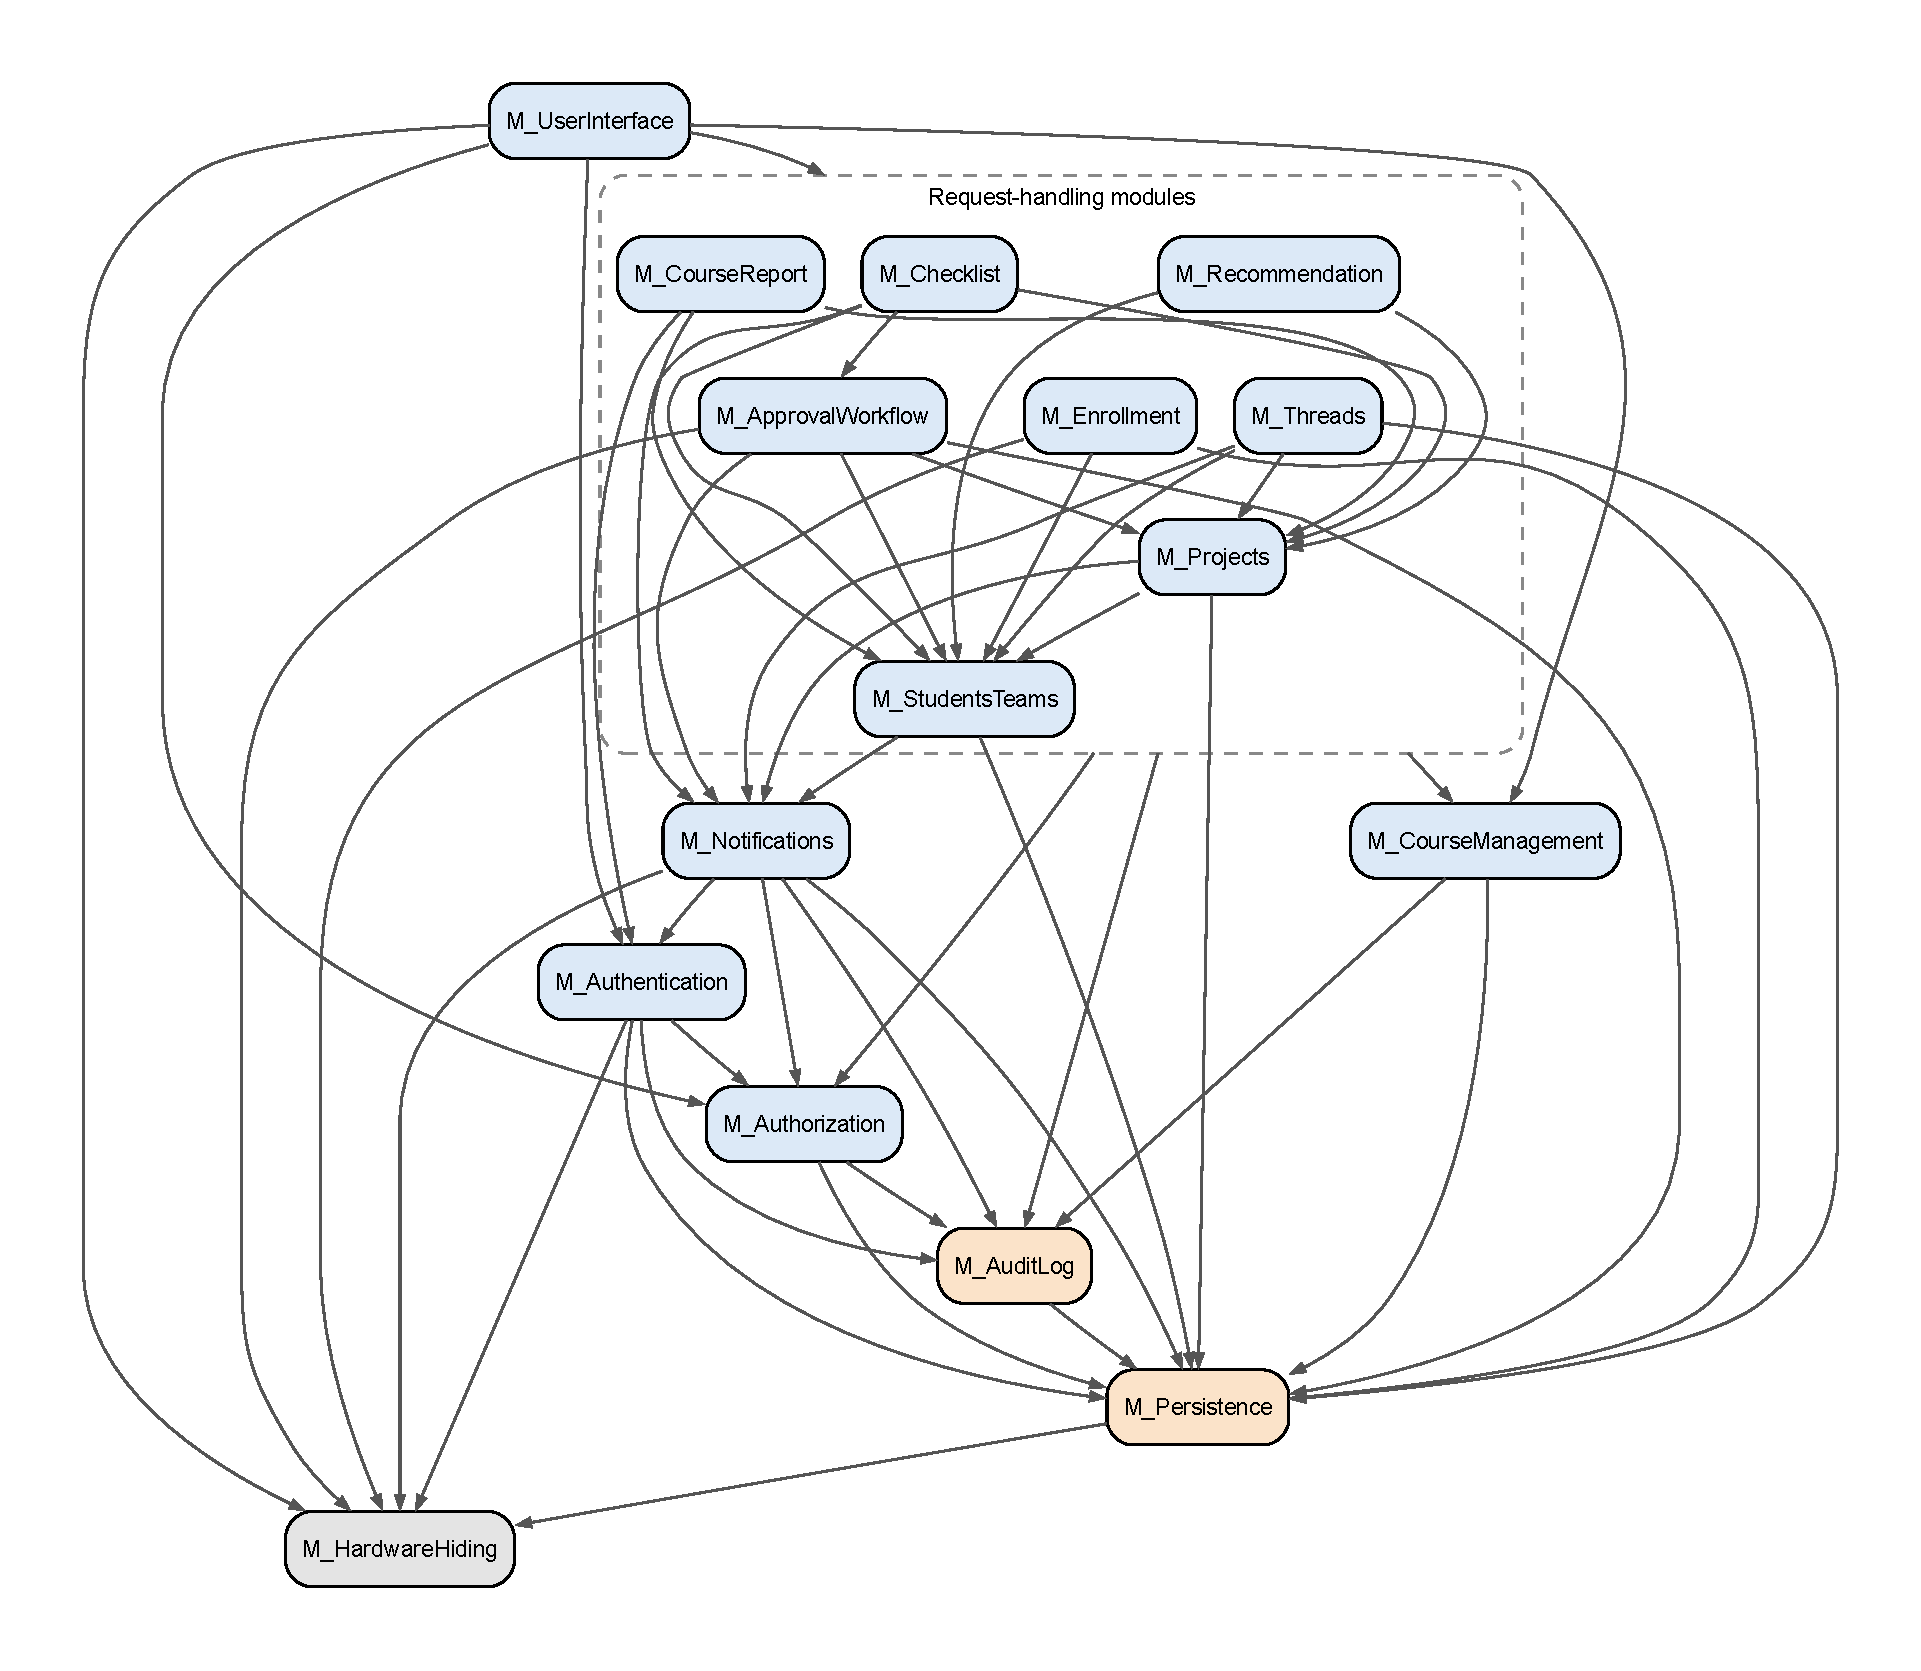
\includegraphics[width=\textwidth,height=0.8\textheight,keepaspectratio]{UsesHierarchy.pdf}%
}{%
  \fbox{\parbox{0.8\textwidth}{\centering UsesHierarchy.pdf is rendered from
  UsesHierarchy.dot by the build. Install Graphviz to render it locally.}}%
}
\caption{Use hierarchy among modules}
\label{FigUH}
\end{figure}

%\section*{References}

\section{User Interfaces}

...to be completed in Revision 0.

\wss{Design of user interface for software and hardware.  Attach an appendix if
needed. Drawings, Sketches, Figma}

\section{Design of Communication Protocols}

...to be completed in Revision 0.

\wss{If there is communication between hardware and software, it may be necessary 
to explain the design of the communication protocol.  This section should be filled 
in with NA if it is not appropriate for a given project.}

\section{Database Design}

...to be completed in Revision 0.

\wss{If a database is a significant component of the project, the database
design should be summarized here.  This section should be filled in with NA if
it is not appropriate for a given project.}

\section{Timeline}

...to be completed in Revision 0.

\wss{Schedule of tasks and who is responsible}

\wss{You can point to GitHub if this information is included there}

\section{Generative AI Use Disclosure}

\wss{ChatGPT (version 5) was used to brainstorm ideas for the template for this disclose section.}

\subsection{AI Tools Used}

\wss{Give the name of the AI tool(s) used and the version.}

\subsection{How and Where Used}

\wss{Explain what the tool(s) were used for.  Examples include: brainstorming,
explaining a technical concept, reviewing the document, generating or modifying
text, generating or modifying diagrams, identifying errors or omissions or
inconsistencies.}

\wss{For each of the uses, identify which parts of the document were affected.}

\wss{You do not need to report every interaction, but you should disclose the 
uses that materially contributed to your work}

\subsection{Verification of AI-Generated Content}

\wss{\begin{itemize}
    \item Describe how the team checked AI-generated or AI-assisted material
    before including it in the document.
    \item In particular, verify factual claims, technical assertions,
    requirements, calculations, references, and other information for which an
    AI system may produce incorrect or fabricated results.
    \item \textbf{The team is responsible for the accuracy, completeness,
consistency, and appropriateness of the submitted document, regardless of
whether material was generated by a human or an AI system.}
\end{itemize}}

\newpage{}

\bibliographystyle {plainnat}
\bibliography{../../../refs/References}

\end{document}
